\documentclass[aspectratio=169,9pt]{beamer}

% base
\usepackage[utf8]{inputenc}
\usepackage[T1]{fontenc}
\usepackage[spanish]{babel}
\usepackage{estilo}
\usetikzlibrary{positioning,arrows.meta,babel}
\graphicspath{{Imagenes/}}

% fuente
\setbeamerfont{frametitle}{size=\Large,series=\bfseries}
\setbeamerfont{title}{size=\LARGE,series=\bfseries}
\setbeamerfont{block title}{size=\small,series=\bfseries}
\setbeamerfont{block body}{size=\small}
\hfuzz=8pt

% datos
\title{Estabilidad Térmica vs. Eficiencia Catalítica}
\subtitle{¿Puede la ingeniería enzimática mejorar ambas propiedades en biocatalizadores industriales?}
\author{Andy Edu Villalobos Melendez}
\institute{Pontificia Universidad Católica del Perú}
\date{}

% imagen
\newcommand{\img}[2]{%
\IfFileExists{Imagenes/#1}{%
\centering\includegraphics[width=\linewidth,height=#2,keepaspectratio]{#1}%
}{%
\begin{beamercolorbox}[wd=\linewidth,ht=#2,dp=0ex,center,rounded=true]{block body}
\vfill{\color{Cian}\bfseries #1}\vfill
\end{beamercolorbox}%
}}

% nav
\newcommand{\boton}[2]{\hyperlink{#1}{\beamerbutton{\fontsize{5.5}{6.2}\selectfont #2}}}
\newcommand{\piecell}[3]{%
\begingroup\setlength{\fboxsep}{1pt}%
\ifnum\value{section}=#1
\hyperlink{#2}{\colorbox{CianClaro}{\parbox[c][0.29cm][c]{0.135\paperwidth}{\centering\color{Fondo}\fontsize{4.9}{5.5}\selectfont\bfseries #3}}}%
\else
\hyperlink{#2}{\colorbox{Cian}{\parbox[c][0.29cm][c]{0.135\paperwidth}{\centering\color{Texto}\fontsize{4.9}{5.5}\selectfont\bfseries #3}}}%
\fi\endgroup}

% footer
\setbeamertemplate{footline}{%
\leavevmode
\begin{beamercolorbox}[wd=\paperwidth,ht=0.46cm,dp=0.07cm,leftskip=0.20cm,rightskip=0.20cm]{normal text}
\vspace{0.04cm}
\piecell{1}{inicio}{Introducción}\hspace{0.04cm}
\piecell{2}{metodologia}{Metodología}\hspace{0.04cm}
\piecell{3}{resultados}{Resultados}\hspace{0.04cm}
\piecell{4}{explotacion}{Explotación}\hspace{0.04cm}
\piecell{5}{conclusion}{Conclusión}
\hfill{\color{TextoSuave}\fontsize{5.4}{6}\selectfont\insertpagenumber/\insertpresentationendpage}
\end{beamercolorbox}}

% doc
\begin{document}

% intro
\section{Introducción}
\subsection{Problema y Pregunta}
\begin{frame}[label=inicio]{Introducción}

\centering
{\color{Cian}\bfseries Problema Industrial}\par
\vspace{0.05cm}
{\Large\bfseries Estabilidad Térmica vs. Eficiencia Catalítica}\par
\vspace{0.03cm}
{\scriptsize\color{TextoSuave}Biocatalizadores industriales: durar más sin convertir peor}

\vspace{0.14cm}
\begin{alertblock}{Pregunta Central}
\centering
\small\bfseries
¿Aumentar la termoestabilidad reduce necesariamente la eficiencia catalítica?
\end{alertblock}

\vspace{0.09cm}
\begin{columns}[T,onlytextwidth]
\column{0.31\textwidth}
\tarjeta{Estabilidad}{\centering Vida operativa\\$t_{50}$ + actividad residual}
\column{0.31\textwidth}
\tarjeta{Eficiencia}{\centering Conversión\\$V_{\max}/K_m$}
\column{0.31\textwidth}
\tarjeta{Producción}{\centering Resultado final\\producto acumulado}
\end{columns}

\vspace{0.10cm}
\begin{beamercolorbox}[wd=0.86\textwidth,sep=0.10cm,rounded=true,center]{block body}
\small\bfseries\color{CianClaro}
Estabilidad $+$ Eficiencia $+$ Operación $\longrightarrow$ Producción Útil
\end{beamercolorbox}

\vfill
\fuente{Hou y cols. (2023); Siddiqui (2017).}
\end{frame}

\subsection{Resumen}
\begin{frame}{Introducción \hfill{\tiny\color{TextoSuave}\textbf{WT}: enzima original \quad | \quad \textbf{ENG}: enzima modificada por ingeniería}}



{\color{Cian}\bfseries Resumen de la Sección}\par
\vspace{0.08cm}

\begin{columns}[T,onlytextwidth]
\column{0.47\textwidth}
\begin{block}{Qué se Sabe}
\small
\begin{itemize}[<+->]
\item Más estabilidad puede restringir movilidad catalítica.
\item El trade-off existe, pero no es una regla obligatoria.
\end{itemize}
\end{block}

\column{0.49\textwidth}
\begin{beamercolorbox}[wd=\linewidth,sep=0.13cm,rounded=true]{block body}
\small
\textbf{Qué se Va a Probar}
\begin{itemize}
\item WT frente a ENG.
\item Estabilidad, eficiencia y producción.
\item Cuatro aplicaciones industriales.
\end{itemize}
\end{beamercolorbox}
\end{columns}

\vspace{0.10cm}
\uncover<3->{
\begin{alertblock}{Idea de Partida}
\centering\small\bfseries
La variante útil no es la que solo dura más: es la que convierte esa mejora en producto.
\end{alertblock}
}

\vfill
\only<3->{
\begin{columns}[b,onlytextwidth]
\column{0.72\textwidth}
\fuente{Hou y cols. (2023); Siddiqui (2017).}
\column{0.24\textwidth}
\raggedleft\boton{metodologia}{Siguiente: Metodología}
\end{columns}}
\end{frame}


% metodo
\section{Metodología}
\subsection{Variables e Indicadores}
\begin{frame}[label=metodologia]{Metodología \hfill{\tiny\color{TextoSuave}\textbf{WT}: enzima original \quad | \quad \textbf{ENG}: enzima modificada por ingeniería}}



{\color{Cian}\bfseries Variables e Indicadores}\par
\vspace{0.08cm}

\begin{columns}[T,onlytextwidth]
\column{0.31\textwidth}
\tarjeta{X · Termoestabilidad}{\centering $t_{50}$\\actividad residual\\\vspace{0.04cm}\textbf{¿Cuánto dura?}}
\column{0.31\textwidth}
\tarjeta{Y · Eficiencia}{\centering $V_{\max}/K_m$\\respuesta al sustrato\\\vspace{0.04cm}\textbf{¿Qué tan bien convierte?}}
\column{0.31\textwidth}
\tarjeta{Resultado · Producción}{\centering producto acumulado\\8 horas\\\vspace{0.04cm}\textbf{¿Genera valor?}}
\end{columns}

\vspace{0.11cm}
\begin{columns}[T,onlytextwidth]
\column{0.48\textwidth}
\begin{block}{Índices}
\small
\begin{itemize}
\item \textbf{IS}: estabilidad ENG / WT.
\item \textbf{IC}: eficiencia ENG / WT.
\item \textbf{IP}: producción ENG / WT.
\end{itemize}
\end{block}
\column{0.48\textwidth}
\begin{alertblock}{Lectura}
\centering\small\bfseries
$>1$ mejora \qquad $=1$ igual \qquad $<1$ empeora
\end{alertblock}
\end{columns}

\vspace{0.06cm}
\begin{beamercolorbox}[wd=\linewidth,sep=0.08cm,rounded=true,center]{block body}
\small\bfseries\color{CianClaro}
Medición Molecular $\longrightarrow$ Comparación WT--ENG $\longrightarrow$ Resultado Productivo
\end{beamercolorbox}

\vfill
\fuente{Hou y cols. (2023); Siddiqui (2017).}
\end{frame}

\subsection{Diseño y Protocolo}
\begin{frame}{Metodología \hfill{\tiny\color{TextoSuave}\textbf{WT}: enzima original \quad | \quad \textbf{ENG}: enzima modificada por ingeniería}}



{\color{Cian}\bfseries Diseño y Protocolo}\par
\vspace{0.07cm}

\begin{columns}[T,onlytextwidth]
\column{0.44\textwidth}
\begin{block}{4 Aplicaciones}
\small
\begin{itemize}
\item Alimentos $\rightarrow$ proteasa.
\item Bagazo $\rightarrow$ $\beta$-glucosidasa.
\item Biomasa $\rightarrow$ xilanasa.
\item Glucósidos $\rightarrow$ $\beta$-glucosidasa.
\end{itemize}
\end{block}

\column{0.48\textwidth}
\begin{block}{Protocolo Común}
\scriptsize
\begin{tabularx}{\linewidth}{@{}>{\bfseries}lY@{}}
Estabilidad & 60 $^{\circ}$C, 10 mM $\rightarrow t_{50}$\\[0.04cm]
Cinética & 0.5--80 mM $\rightarrow$ eficiencia\\[0.04cm]
Temperatura & 35--90 $^{\circ}$C $\rightarrow T_{opt}$\\[0.04cm]
Producción & 60 $^{\circ}$C, 40 mM, 8 h\\[0.04cm]
Exploración & misma malla $\rightarrow$ mejor punto
\end{tabularx}
\end{block}
\end{columns}

\vspace{0.11cm}
\begin{block}{Secuencia de Decisión}
\centering
\resizebox{0.80\linewidth}{!}{%
\begin{tikzpicture}[>=Latex,node distance=0.10cm]
\tikzset{n/.style={draw=Linea,fill=PanelDos,rounded corners=2pt,text=Texto,minimum height=0.55cm,inner xsep=0.10cm,font=\scriptsize\bfseries}}
\node[n] (a) {WT vs. ENG};
\node[n,right=of a] (b) {Medir};
\node[n,right=of b] (c) {Comparar};
\node[n,right=of c] (d) {Detectar};
\node[n,right=of d] (e) {Optimizar};
\draw[->,Cian] (a)--(b);\draw[->,Cian] (b)--(c);\draw[->,Cian] (c)--(d);\draw[->,Cian] (d)--(e);
\end{tikzpicture}%
}
\end{block}

\vfill
\fuente{4 réplicas por condición.}
\end{frame}

\subsection{Resumen}
\begin{frame}{Metodología \hfill{\tiny\color{TextoSuave}\textbf{WT}: enzima original \quad | \quad \textbf{ENG}: enzima modificada por ingeniería}}



{\color{Cian}\bfseries Resumen de la Sección}\par
\vspace{0.08cm}

\begin{columns}[T,onlytextwidth]
\column{0.31\textwidth}
\tarjeta{Qué se Hizo}{\centering Misma lógica WT--ENG\\en cuatro procesos}
\column{0.31\textwidth}
\tarjeta{Cómo se Midió}{\centering IS + IC + IP\\temperatura + sustrato}
\column{0.31\textwidth}
\tarjeta{Por Qué}{\centering Separar mejora molecular\\de mejora productiva}
\end{columns}

\vspace{0.13cm}
\begin{alertblock}{Criterio de Éxito}
\centering\small\bfseries
ENG debe durar más, convertir mejor y producir más sin crear un nuevo límite dominante.
\end{alertblock}

\vspace{0.10cm}
\begin{beamercolorbox}[wd=\linewidth,sep=0.10cm,rounded=true,center]{block body}
\small\bfseries\color{CianClaro}
Estabilidad $\uparrow$ + Eficiencia $\uparrow$ $\not\Rightarrow$ valor automático
\qquad
Operación correcta $\Rightarrow$ valor capturable
\end{beamercolorbox}

\vfill
\begin{columns}[b,onlytextwidth]
\column{0.23\textwidth}
\boton{inicio}{Anterior: Introducción}
\column{0.52\textwidth}
\column{0.23\textwidth}
\raggedleft\boton{resultados}{Siguiente: Resultados}
\end{columns}
\end{frame}


% resultados
\section{Resultados}
\subsection{Termoestabilidad}
\begin{frame}[label=resultados]{Resultados \hfill{\tiny\color{TextoSuave}\textbf{WT}: enzima original \quad | \quad \textbf{ENG}: enzima modificada por ingeniería}}



{\color{Cian}\bfseries Termoestabilidad: ENG Extiende la Vida Operativa}\par
\vspace{0.06cm}

\begin{columns}[T,onlytextwidth]
\column{0.60\textwidth}
\img{2.png}{0.48\textheight}

\column{0.36\textwidth}
\begin{beamercolorbox}[wd=\linewidth,sep=0.12cm,rounded=true]{block body}
\small
\textbf{$t_{50}$ WT $\rightarrow$ ENG}
\begin{itemize}
\item Alimentos: 1.11 $\rightarrow$ 3.53 h.
\item \textbf{Bagazo: 0.75 $\rightarrow$ 7.02 h.}
\item Biomasa: 0.99 $\rightarrow$ 6.13 h.
\item Glucósidos: 1.49 $\rightarrow$ 5.43 h.
\end{itemize}
\end{beamercolorbox}

\vspace{0.08cm}
\begin{alertblock}{Mayor Ganancia}
\centering\small\bfseries
Bagazo: IS = 6.92
\end{alertblock}
\end{columns}

\vspace{0.07cm}
\begin{block}{Lectura}
\centering\small
ENG cruza el 50\% de actividad mucho más tarde: \textbf{la vida operativa aumenta en los cuatro casos}.
\end{block}
\end{frame}

\subsection{Eficiencia y Temperatura}
\begin{frame}{Resultados \hfill{\tiny\color{TextoSuave}\textbf{WT}: enzima original \quad | \quad \textbf{ENG}: enzima modificada por ingeniería}}



{\color{Cian}\bfseries Eficiencia Catalítica y Temperatura Óptima}\par
\vspace{0.06cm}

\begin{columns}[T,onlytextwidth]
\column{0.47\textwidth}
{\scriptsize\bfseries\color{Texto}Eficiencia ENG / WT}\par\vspace{0.04cm}
\img{19.png}{0.39\textheight}

\column{0.49\textwidth}
{\scriptsize\bfseries\color{Texto}Respuesta Térmica · Biomasa}\par\vspace{0.04cm}
\img{11.png}{0.39\textheight}
\end{columns}

\vspace{0.08cm}
\begin{columns}[T,onlytextwidth]
\column{0.48\textwidth}
\begin{block}{IC}
\centering\scriptsize
Alimentos 1.54 $\times$ \quad Bagazo 1.48 $\times$\\
Biomasa 1.58 $\times$ \quad \textbf{Glucósidos 2.56 $\times$}
\end{block}
\column{0.48\textwidth}
\begin{alertblock}{$T_{opt}$ WT $\rightarrow$ ENG}
\centering\scriptsize
Alimentos 60$\rightarrow$65 $^{\circ}$C \quad Bagazo 55$\rightarrow$65 $^{\circ}$C\\
Biomasa 65$\rightarrow$75 $^{\circ}$C \quad Glucósidos 55$\rightarrow$60 $^{\circ}$C
\end{alertblock}
\end{columns}
\end{frame}

\subsection{Producción}
\begin{frame}{Resultados \hfill{\tiny\color{TextoSuave}\textbf{WT}: enzima original \quad | \quad \textbf{ENG}: enzima modificada por ingeniería}}



{\color{Cian}\bfseries Producción: la Mejora Molecular Sí Llega al Proceso}\par
\vspace{0.06cm}

\begin{columns}[T,onlytextwidth]
\column{0.62\textwidth}
\img{20.png}{0.50\textheight}

\column{0.34\textwidth}
\begin{beamercolorbox}[wd=\linewidth,sep=0.12cm,rounded=true]{block body}
\small
\textbf{IP · condición base}
\begin{itemize}
\item Alimentos: 4.58$\times$.
\item Bagazo: 8.96$\times$.
\item Biomasa: 5.41$\times$.
\item \textbf{Glucósidos: 15.29$\times$.}
\end{itemize}
\end{beamercolorbox}

\vspace{0.08cm}
\begin{block}{Base Común}
\centering\small
60 $^{\circ}$C | 40 mM | 8 h
\end{block}
\end{columns}

\vspace{0.07cm}
\begin{alertblock}{Resultado Directo}
\centering\small\bfseries
ENG produjo más que WT en los cuatro procesos; glucósidos mostró la mayor amplificación.
\end{alertblock}
\end{frame}

\subsection{Resumen}
\begin{frame}[label=resumen_resultados]{Resultados \hfill{\tiny\color{TextoSuave}\textbf{WT}: enzima original \quad | \quad \textbf{ENG}: enzima modificada por ingeniería}}

{\color{Cian}\bfseries Resumen de la Sección}

\vspace{0.05cm}

\begin{columns}[T,onlytextwidth]

\column{0.50\textwidth}

{\color{CianClaro}\bfseries Síntesis Estabilidad--Eficiencia}

\vspace{0.04cm}

\centering
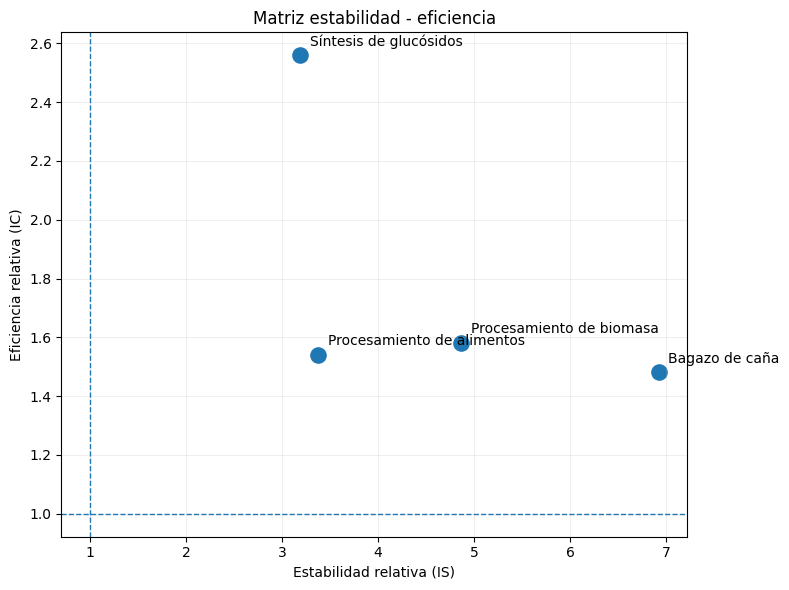
\includegraphics[
    width=\linewidth,
    height=0.42\textheight,
    keepaspectratio
]{21.png}

\vspace{0.05cm}

\begin{block}{Qué se Hizo}
\scriptsize
Se integraron \textbf{estabilidad, eficiencia, producción y temperatura óptima} para comparar WT frente a ENG.
\end{block}


\column{0.47\textwidth}

{\color{CianClaro}\bfseries Hallazgos Clave}

\vspace{0.04cm}

\begin{beamercolorbox}[
    wd=\linewidth,
    sep=0.10cm,
    rounded=true
]{block body}

\scriptsize

\begin{itemize}
    \item \textbf{Bagazo:} mayor estabilidad
    \hfill IS = \textbf{6.92}

    \item \textbf{Glucósidos:} mayor eficiencia
    \hfill IC = \textbf{2.56}

    \item \textbf{Glucósidos:} mayor producción base
    \hfill IP = \textbf{15.29}

    \item \textbf{Biomasa:} mayor desplazamiento térmico
    \hfill 65 $\rightarrow$ 75 $^{\circ}$C
\end{itemize}

\end{beamercolorbox}

\vspace{0.07cm}

\begin{alertblock}{Resultado Central}
\centering
\scriptsize\bfseries

IS $>1$ e IC $>1$ en los cuatro procesos.

\vspace{0.03cm}

La mayor termoestabilidad \textbf{no exigió sacrificar eficiencia catalítica}.
\end{alertblock}

\end{columns}

\vspace{0.05cm}

\begin{beamercolorbox}[
    wd=\linewidth,
    sep=0.07cm,
    rounded=true,
    center
]{block body}
\scriptsize
\textbf{La enzima modificada superó a la original en los cuatro casos,}
pero cada proceso presentó un cuello de botella diferente.
\end{beamercolorbox}

\vfill

\begin{columns}[b,onlytextwidth]

\column{0.24\textwidth}
\boton{metodologia}{Anterior: Metodología}

\column{0.50\textwidth}

\column{0.24\textwidth}
\raggedleft
\boton{explotacion}{Siguiente: Explotación}

\end{columns}

\end{frame}

% explotacion
\section{Explotación}
\subsection{Cuellos de Botella}
\begin{frame}[label=explotacion]{Explotación \hfill{\tiny\color{TextoSuave}\textbf{WT}: enzima original \quad | \quad \textbf{ENG}: enzima modificada por ingeniería}}



{\color{Cian}\bfseries Cuellos de Botella: Qué Limita Cada Proceso}\par
\vspace{0.06cm}

\begin{columns}[T,onlytextwidth]
\column{0.48\textwidth}
{\scriptsize\bfseries\color{Texto}Bagazo · Inhibición por Producto}\par\vspace{0.04cm}
\img{23.png}{0.35\textheight}

\column{0.48\textwidth}
{\scriptsize\bfseries\color{Texto}Glucósidos · Inhibición por Sustrato}\par\vspace{0.04cm}
\img{25.png}{0.35\textheight}
\end{columns}

\vspace{0.05cm}
\begin{columns}[T,onlytextwidth]
\column{0.48\textwidth}
\begin{block}{Mapa de Límites}
\scriptsize
\begin{itemize}
\item Alimentos $\rightarrow$ inactivación temprana.
\item Bagazo $\rightarrow$ glucosa acumulada.
\end{itemize}
\end{block}
\column{0.48\textwidth}
\begin{block}{Mapa de Límites}
\scriptsize
\begin{itemize}
\item Biomasa $\rightarrow$ ventana térmica.
\item Glucósidos $\rightarrow$ sustrato + selectividad.
\end{itemize}
\end{block}
\end{columns}

\vspace{0.02cm}
\begin{alertblock}{Regla de Explotación}
\centering\small\bfseries
Mejorar ENG $\rightarrow$ identificar el nuevo límite $\rightarrow$ ajustar temperatura y sustrato.
\end{alertblock}
\end{frame}

\subsection{Puntos de Operación y Valor}
\begin{frame}{Explotación \hfill{\tiny\color{TextoSuave}\textbf{WT}: enzima original \quad | \quad \textbf{ENG}: enzima modificada por ingeniería}}



{\color{Cian}\bfseries Puntos de Operación y Captura de Valor}\par
\vspace{0.01cm}

\begin{beamercolorbox}[wd=\linewidth,sep=0.06cm,rounded=true]{block body}
\centering
\resizebox{0.97\linewidth}{!}{%
\begin{tabular}{@{}lccccc@{}}
\toprule
\textbf{Aplicación} & \textbf{ENG: T,S} & \textbf{Prod.} & \textbf{WT: T,S} & \textbf{Prod.} & \textbf{Ventaja}\\
\midrule
Alimentos & 60 $^{\circ}$C, 40 mM & 16.47 & 45 $^{\circ}$C, 40 mM & 5.93 & 2.78$\times$\\
Bagazo & 60 $^{\circ}$C, 40 mM & 12.70 & 45 $^{\circ}$C, 20 mM & 2.93 & 4.33$\times$\\
Biomasa & 70 $^{\circ}$C, 80 mM & 36.04 & 50 $^{\circ}$C, 40 mM & 7.38 & 4.88$\times$\\
Glucósidos & 60 $^{\circ}$C, 40 mM & 9.49 & 45 $^{\circ}$C, 20 mM & 1.59 & \textbf{5.95$\times$}\\
\bottomrule
\end{tabular}%
}
\end{beamercolorbox}

\vspace{0.03cm}
\begin{columns}[T,onlytextwidth]
\column{0.48\textwidth}
\begin{alertblock}{Mayor Potencial Productivo}
\centering\footnotesize\bfseries
Glucósidos · 60 $^{\circ}$C · 40 mM · 8 h\\
5.95$\times$ vs. mejor WT
\end{alertblock}

\column{0.48\textwidth}
\begin{block}{Cómo Convertirlo en Dinero}
\centering\footnotesize
$\Delta$Producto $\times$ Precio $-$ ENG $-$ Energía\\
$=$ \textbf{Margen incremental}
\end{block}
\end{columns}

\vspace{0.02cm}
\begin{beamercolorbox}[wd=\linewidth,sep=0.05cm,rounded=true,center]{block body}
\scriptsize \textbf{Biomasa:} actividad máxima $\approx75^{\circ}$C; producción máxima $\approx70^{\circ}$C $\Rightarrow$ optimizar producto.
\end{beamercolorbox}
\end{frame}

\subsection{Resumen}
\begin{frame}{Explotación \hfill{\tiny\color{TextoSuave}\textbf{WT}: enzima original \quad | \quad \textbf{ENG}: enzima modificada por ingeniería}}



{\color{Cian}\bfseries Resumen de la Sección}\par
\vspace{0.07cm}

\begin{columns}[T,onlytextwidth]
\column{0.47\textwidth}
\begin{block}{Qué Hacer}
\small
\begin{enumerate}
\item \textbf{Glucósidos:} 60 $^{\circ}$C, 40 mM $\rightarrow$ producto útil + selectividad.
\item \textbf{Biomasa:} 70 $^{\circ}$C, 80 mM $\rightarrow$ explotar ventana térmica.
\item \textbf{Bagazo:} 60 $^{\circ}$C, 40 mM $\rightarrow$ estabilidad + tolerancia.
\item \textbf{Alimentos:} 60 $^{\circ}$C, 40 mM $\rightarrow$ vida operativa.
\end{enumerate}
\end{block}

\column{0.49\textwidth}
\begin{alertblock}{Prioridad Productiva}
\centering\small\bfseries
Glucósidos 5.95$\times$\\
$>$ Biomasa 4.88$\times$\\
$>$ Bagazo 4.33$\times$\\
$>$ Alimentos 2.78$\times$
\end{alertblock}

\vspace{0.08cm}
\begin{beamercolorbox}[wd=\linewidth,sep=0.10cm,rounded=true]{block body}
\scriptsize
\textbf{Por qué:} glucósidos combina IC = 2.56 con selectividad/tolerancia; FP = 1.87 amplifica la mejora molecular.
\end{beamercolorbox}
\end{columns}

\vspace{0.08cm}
\begin{block}{Lectura Económica}
\centering\small
Con los datos actuales se identifica \textbf{potencial productivo}. La rentabilidad neta se confirma con precio, costo ENG y energía.
\end{block}

\vfill
\begin{columns}[b,onlytextwidth]
\column{0.23\textwidth}
\boton{resultados}{Anterior: Resultados}
\column{0.52\textwidth}
\column{0.23\textwidth}
\raggedleft\boton{conclusion}{Siguiente: Conclusión}
\end{columns}
\end{frame}


% cierre
\section{Conclusión}
\subsection{Decisión Final}
\begin{frame}[label=conclusion]{Conclusión \hfill{\tiny\color{TextoSuave}\textbf{WT}: enzima original \quad | \quad \textbf{ENG}: enzima modificada por ingeniería}}

{\color{Cian}\bfseries Decisión Final}

\vspace{0.04cm}

\begin{alertblock}{Respuesta a la Pregunta}
\centering
\scriptsize\bfseries
No. La enzima modificada mejoró simultáneamente
\textbf{termoestabilidad y eficiencia catalítica}
en los cuatro procesos.
\end{alertblock}

\vspace{0.04cm}

\begin{columns}[T,onlytextwidth]

\column{0.49\textwidth}

\begin{block}{1. Prioridad Técnica}
\scriptsize

\begin{itemize}
    \item \textbf{Proceso:} Síntesis de Glucósidos
    \item \textbf{Operación:} 60 $^{\circ}$C, 40 mM, 8 h
    \item \textbf{Ventaja:} \textbf{5.95$\times$} frente a WT
    \item \textbf{Motor:} eficiencia + selectividad
\end{itemize}

\centering
{\color{CianClaro}\bfseries Mayor Potencial Productivo}
\end{block}


\column{0.49\textwidth}

\begin{block}{2. Segunda Prioridad}
\scriptsize

\begin{itemize}
    \item \textbf{Proceso:} Biomasa
    \item \textbf{Operación:} 70 $^{\circ}$C, 80 mM, 8 h
    \item \textbf{Ventaja:} \textbf{4.88$\times$} frente a WT
    \item \textbf{Clave:} producir a 70 $^{\circ}$C, no a 75 $^{\circ}$C
\end{itemize}

\centering
{\color{CianClaro}\bfseries Explotar la Ventana Térmica}
\end{block}

\end{columns}

\vspace{0.04cm}

\begin{beamercolorbox}[
    wd=\linewidth,
    sep=0.08cm,
    rounded=true,
    center
]{block body}
\scriptsize\bfseries\color{CianClaro}

Ingeniería Enzimática
$\rightarrow$
Mejora Molecular
$\rightarrow$
Punto Operativo
$\rightarrow$
Mayor Producto Útil

\end{beamercolorbox}

\vspace{0.04cm}

\begin{block}{Recomendación}
\centering
\scriptsize\bfseries

\textbf{Priorizar Síntesis de Glucósidos}

\vspace{0.02cm}

60 $^{\circ}$C
\quad | \quad
40 mM
\quad | \quad
8 h
\quad $\rightarrow$ \quad
\textbf{5.95$\times$}

\vspace{0.02cm}

{\tiny
Primera alternativa para validación industrial por presentar
la mayor ventaja productiva del rango evaluado.
}
\end{block}

\vfill

\boton{explotacion}{Anterior: Explotación}

\end{frame}

\end{document}
